\documentclass[12pt]{article}
\usepackage{amsmath, amssymb, graphicx, hyperref, geometry}
\usepackage{float}
\usepackage{caption}
\usepackage{fancyhdr}
\usepackage{xcolor}
\geometry{margin=1in}
\pagestyle{fancy}
\fancyhf{}
\rhead{GBM Simulation}
\lhead{Quantitative Finance}
\rfoot{Page \thepage}

\title{Stock Price Simulation using Geometric Brownian Motion}
\author{Naimish Pintukumar Machchhar}
\date{\today}

\begin{document}

\maketitle

\tableofcontents
\newpage

%---------------------------
\section{Introduction}
In quantitative finance, modeling the stochastic behavior of asset prices is foundational for derivative pricing, risk assessment, and portfolio simulation. This report focuses on simulating stock prices using the \textbf{Geometric Brownian Motion (GBM)} model—a continuous-time stochastic process widely used in financial mathematics, especially in the Black-Scholes framework.

The project aims to:
\begin{itemize}
    \item Understand the assumptions and derivation of GBM
    \item Implement GBM simulation using Python
    \item Generate and visualize both single and multiple price paths
    \item Analyze the statistical distribution of outcomes
\end{itemize}

%---------------------------
\section{Theory: Stochastic Processes and GBM}

\subsection{Brownian Motion (Wiener Process)}
Brownian motion \( W_t \) is a continuous-time stochastic process with:
\begin{itemize}
    \item \( W_0 = 0 \)
    \item Independent and normally distributed increments
    \item \( W_t - W_s \sim \mathcal{N}(0, t - s) \)
    \item Continuous but nowhere differentiable paths
\end{itemize}

\subsection{Geometric Brownian Motion}
GBM models stock prices with the stochastic differential equation:
\[
dS_t = \mu S_t \, dt + \sigma S_t \, dW_t
\]
where:
\begin{itemize}
    \item \( S_t \): stock price at time \( t \)
    \item \( \mu \): expected return (drift)
    \item \( \sigma \): volatility
    \item \( W_t \): Brownian motion
\end{itemize}

The solution to this SDE is:
\[
S_t = S_0 \exp\left[\left(\mu - \frac{1}{2} \sigma^2\right)t + \sigma W_t\right]
\]

%---------------------------
\section{Implementation Overview (Python Simulation Steps)}

The simulation was implemented in Python using NumPy and Matplotlib. Below is the step-by-step logic of how the GBM simulation was structured in code.

\subsection{Set Initial Parameters}
Parameters were defined:
\begin{itemize}
    \item Initial stock price \( S_0 \)
    \item Drift \( \mu \)
    \item Volatility \( \sigma \)
    \item Time horizon \( T \) in years
    \item Number of time steps \( N \)
    \item Number of simulations \( M \)
\end{itemize}

\subsection{Create Time Grid}
A time grid was constructed from \( t = 0 \) to \( t = T \) with step size:
\[
\Delta t = \frac{T}{N}
\]

\subsection{Simulate Brownian Motion}
\begin{itemize}
    \item Generate standard normal random variables \( Z \sim \mathcal{N}(0,1) \)
    \item Multiply by \( \sqrt{\Delta t} \) to scale
    \item Cumulatively sum to generate Brownian paths
\end{itemize}

\subsection{Apply GBM Formula}
Using the analytical GBM solution:
\[
S_t = S_0 \exp\left[\left(\mu - \frac{1}{2} \sigma^2\right)t + \sigma W_t\right]
\]
This was vectorized for both single and multiple simulations.

\subsection{Plot a Single Simulated Path}
A single GBM path was visualized to observe the stochastic price movement:

\begin{figure}[H]
    \centering
    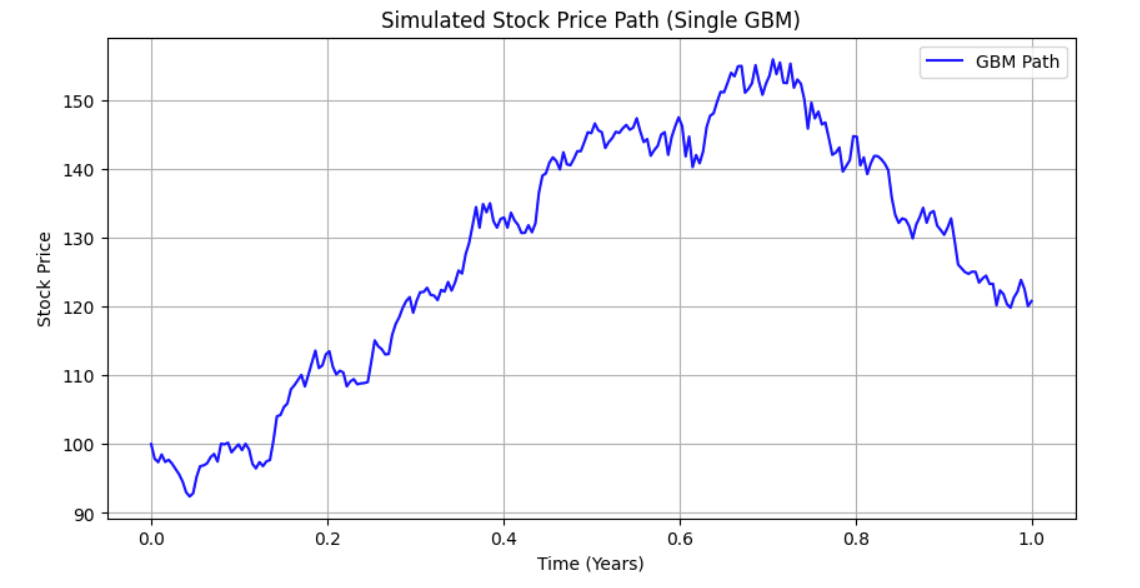
\includegraphics[width=0.85\textwidth]{Single Path Simulation.png}
    \caption{Simulated Stock Price (Single GBM Path)}
\end{figure}

\subsection{Monte Carlo Simulation}
\begin{itemize}
    \item \( M \) (1000) paths were simulated simultaneously
    \item The paths were plotted together to visualize spread and volatility
\end{itemize}

\begin{figure}[H]
    \centering
    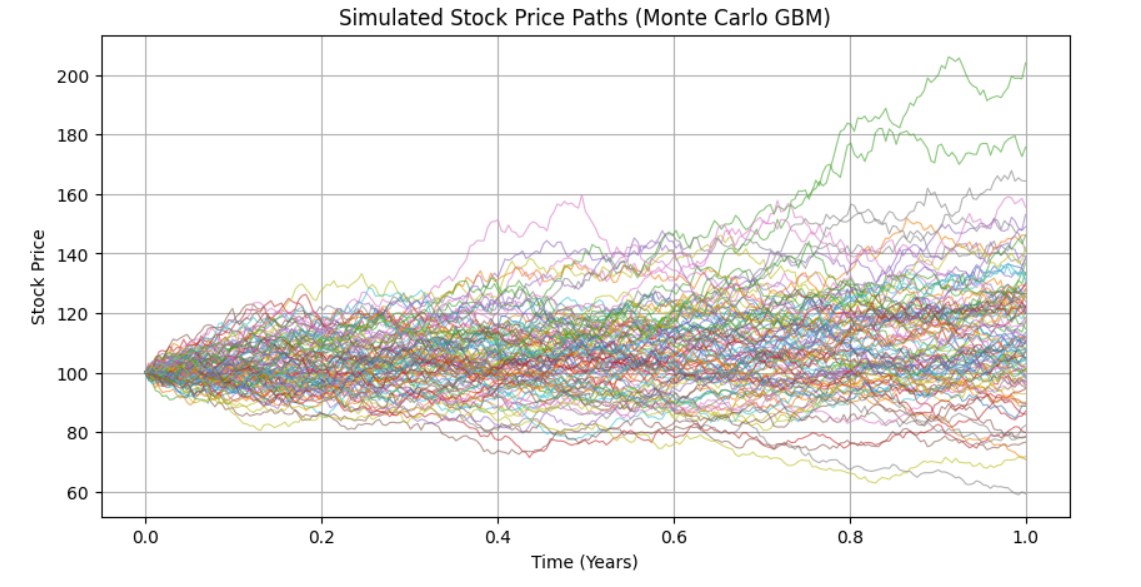
\includegraphics[width=0.85\textwidth]{Monte Carlo Simulation.png}
    \caption{Monte Carlo Simulation with 1000 GBM Paths (Exemplary 100 Paths)}
\end{figure}


\section{Monte Carlo Analysis: Mean Path and Confidence Bands}

Beyond observing individual simulation paths or final price distributions, it's insightful to aggregate results statistically across all Monte Carlo paths. This section describes how we visualized the central tendency and dispersion of simulated stock prices over time.

\subsection*{Statistical Summaries Across Simulations}
For each time step, the following statistics were computed across all simulations:
\begin{itemize}
    \item \textbf{Mean Path:} The average stock price at each time point across all simulations
    \item \textbf{10th and 90th Percentiles:} These define a confidence interval band representing the middle 80\% of outcomes
\end{itemize}

\subsection*{Visualization of Central Tendency and Dispersion}
The following visualization was generated:
\begin{itemize}
    \item A bold black line representing the mean stock price over time
    \item A shaded gray band showing the 10th to 90th percentile range (80\% confidence band)
    \item Ten individual simulation paths overlaid with dashed lines to give a qualitative sense of variation
\end{itemize}

\begin{figure}[H]
    \centering
    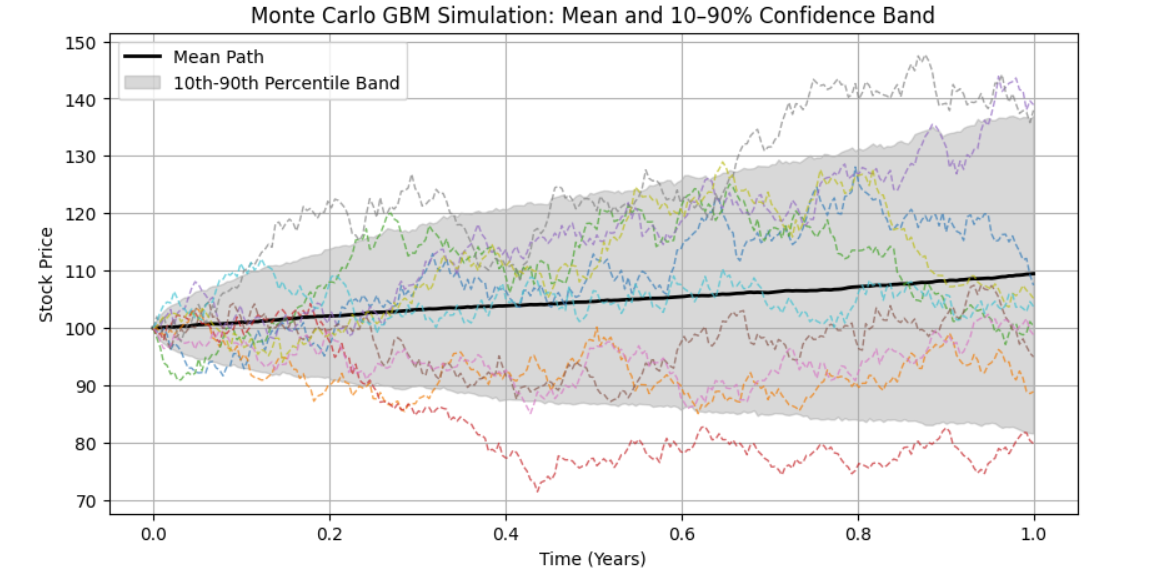
\includegraphics[width=0.85\textwidth]{Mean Path and Confidence Bands.png}
    \caption{Mean GBM Path with 10th–90th Percentile Confidence Band and Sample Paths}
\end{figure}

\subsection*{Interpretation}
\begin{itemize}
    \item The mean path grows exponentially, consistent with the GBM model's expected return.
    \item The width of the percentile band increases with time, reflecting growing uncertainty in price outcomes.
    \item The overlaid sample paths exhibit a wide spread, emphasizing the importance of probabilistic forecasting over deterministic predictions.
\end{itemize}





\section{Histogram of Final Prices}
Final prices \( S_T \) from each simulation were extracted and plotted as a histogram to examine the terminal distribution:

\begin{figure}[H]
    \centering
    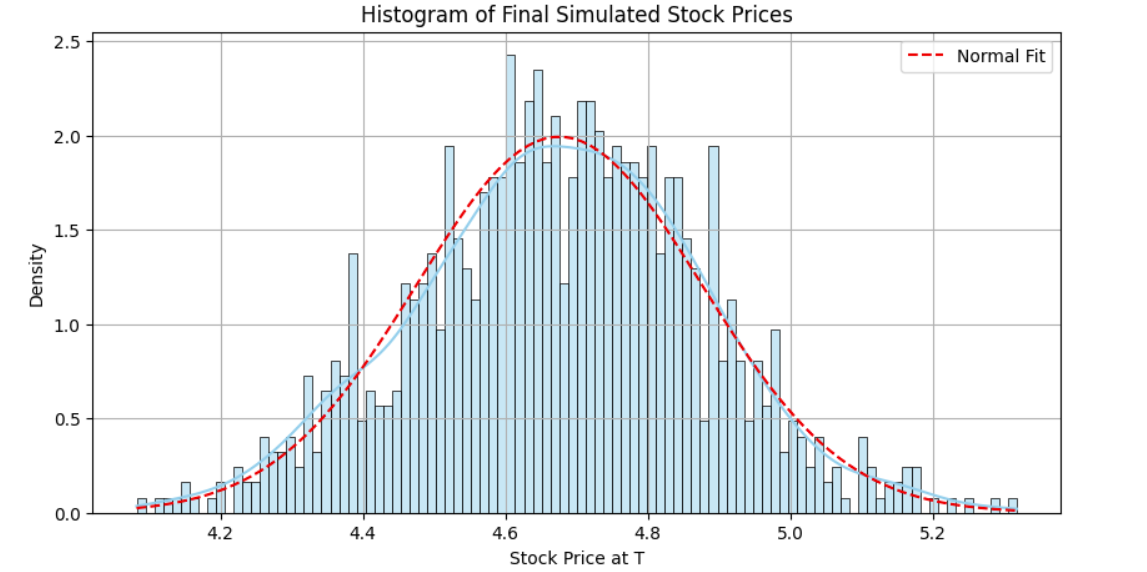
\includegraphics[width=0.85\textwidth]{Final Prices Histogram.png}
    \caption{Histogram of Final Prices at Time \( T \)}
\end{figure}

Optionally, a normal distribution was overlaid to compare against the empirical histogram.

%---------------------------
\section{Observations and Analysis}

\begin{itemize}
    \item The mean trajectory of GBM reflects the influence of drift \( \mu \)
    \item Volatility \( \sigma \) governs the spread between different paths
    \item The final distribution of prices is log-normal, not symmetric
    \item Even with the same initial price and parameters, path outcomes vary significantly
\end{itemize}

%---------------------------
\section{Limitations of GBM}
\begin{itemize}
    \item Assumes constant volatility and drift
    \item Ignores real-world factors like jumps, mean-reversion, or news
    \item Not suitable for predicting real asset prices
    \item Can be improved by using models like:
    \begin{itemize}
        \item Stochastic volatility models (e.g., Heston)
        \item Jump-diffusion models (e.g., Merton)
        \item Machine learning models with historical data
    \end{itemize}
\end{itemize}

%---------------------------
\section{Conclusion}
Geometric Brownian Motion is a fundamental model that captures essential features of stock price dynamics like random variation and drift. While it lacks realism in many aspects, it serves as a stepping stone to more sophisticated modeling techniques in quantitative finance.

This project not only illustrates GBM mathematically but also demonstrates its simulation through clean Pythonic implementation and intuitive visualizations.


\end{document}
